\documentclass[10pt]{article}

% Pacotes extras necessários
\usepackage{amsmath}
\usepackage[lmargin=0.5in, rmargin=0.5in, tmargin=0.5in, bmargin=0.5in, includehead, includefoot]{geometry}
\usepackage{amsfonts}
\usepackage[utf8]{inputenc}
\usepackage[portuguese]{babel}
\usepackage{graphicx}
\usepackage{fancyhdr}
\usepackage{setspace}

\graphicspath{ {./images/} }

% Sets para outras partes
\setlength{\parindent}{0pt}
\setstretch{1.5}
\setcounter{MaxMatrixCols}{15}
\DeclareMathOperator{\sen}{sen}
\DeclareMathOperator{\sinc}{sinc}

%% Facilidades
%% -- Laplace
\newcommand{\Lap}[1]{\mathcal{L}\left\{#1\right\}}

%% -- Fourier
\newcommand{\Fou}[1]{\mathcal{F}\left\{#1\right\}}

%% -- Transformada Z
\newcommand{\Z}[1]{\mathcal{Z}\left\{#1\right\}}

%% -- Negrito em matemáticas
\newcommand{\bm}[1]{\boldsymbol{#1}}

%% -- Haar 
\newcommand{\Ha}[1]{\mathcal{H}\left(#1\right)}

%% -- Haar inversa
\newcommand{\Hi}[1]{\mathcal{H}^{-1}\left(#1\right)}

%% -- Haar de nivel n
\newcommand{\Hn}[2]{\mathcal{H}^{#1}\left(#2\right)}


% ------- Estilo do trabalho -------- %
\fancypagestyle{capa}{
    \fancyhf{}
    \renewcommand\headrulewidth{0pt}
    \fancyfoot[C]{
        Rio de Janeiro\\
        2022
    }
}

\pagestyle{fancy}
\fancyhead{}
\fancyhead[L]{\thepage}
\fancyfoot{}
% ----------------------------------- %

% Dados do Grupo
\title{Sinais e Sistemas - Trabalho 7 - Avaliação 11}
\author{
    \textbf{Grupo 2}\\
    Leonardo Soares da Costa Tanaka\\
    Matheus Henrique Sant Anna Cardoso\\
    Theo Rudra Macedo e Silva\\
    Vinícius Quintanilha Porto Gomes
}
\date{}

\begin{document}
\maketitle
\thispagestyle{capa}
\newpage

\textbf{1.)} Para o sinal abaixo:

\textbf{G2: } $x = [30 \ \ 20 \ \ 12 \ \ 6 \ \ 2 \ \ 0 \ \ 0 \ \ 2 \ \ 6 \ \ 12 \ \ 20 \ \ 30]$

(a) compute a primeira tendência e a primeira flutuação, por Haar;

Aqui, fazemos:
\[\begin{bmatrix}
    30 & 20 & 12 & 6 & 2 & 0 & 0 & 2 & 6 & 12 & 20 & 30
\end{bmatrix}
\cdot \frac{1}{\sqrt{2}} \cdot
\begin{bmatrix}
    1 & 0 & 0 & 0 & 0 & 0 & 1  & 0  & 0  & 0  & 0  & 0 \\
    1 & 0 & 0 & 0 & 0 & 0 & -1 & 0  & 0  & 0  & 0  & 0 \\
    0 & 1 & 0 & 0 & 0 & 0 & 0  & 1  & 0  & 0  & 0  & 0 \\
    0 & 1 & 0 & 0 & 0 & 0 & 0  & -1 & 0  & 0  & 0  & 0 \\
    0 & 0 & 1 & 0 & 0 & 0 & 0  & 0  & 1  & 0  & 0  & 0 \\
    0 & 0 & 1 & 0 & 0 & 0 & 0  & 0  & -1 & 0  & 0  & 0 \\
    0 & 0 & 0 & 1 & 0 & 0 & 0  & 0  & 0  & 1  & 0  & 0 \\
    0 & 0 & 0 & 1 & 0 & 0 & 0  & 0  & 0  & -1 & 0  & 0 \\
    0 & 0 & 0 & 0 & 1 & 0 & 0  & 0  & 0  & 0  & 1  & 0 \\
    0 & 0 & 0 & 0 & 1 & 0 & 0  & 0  & 0  & 0  & -1 & 0 \\
    0 & 0 & 0 & 0 & 0 & 1 & 0  & 0  & 0  & 0  & 0  & 1 \\
    0 & 0 & 0 & 0 & 0 & 1 & 0  & 0  & 0  & 0  & 0  & -1
\end{bmatrix}\]

Obtendo:
\[\sqrt{2} \cdot \begin{bmatrix}
    25 & 9 & 1 & 1 & 9 & 25 & \mid & 5 & 3 & 1 & -1 & -3 & -5
\end{bmatrix}\]
Sendo o sub de tendência: $\sqrt{2} \cdot \begin{bmatrix}
    25 & 9 & 1 & 1 & 9 & 25
\end{bmatrix}$

Sendo o sub de flutuação: $\sqrt{2} \cdot \begin{bmatrix}
    5 & 3 & 1 & -1 & -3 & -5
\end{bmatrix}$

\vspace{1em}

(b) determine a porcentagem de compactação, ou seja, a energia do sub de tendência dividida pela energia total;

Energia do sinal $x$: 2968.

Energia do sub de Tendência: 2828

A porcentagem de compactação $C$ será dada por:
\[C = \frac{2828}{2968}\]
\[\boxed{C = 95.28\%}\]

(c) compute uma aproximação $\tilde{x}$ anulando as primeiras flutuações $(d_i^1 = 0)$;

Anulando as primeiras flutuações, teremos:
\[\sqrt{2} \cdot \begin{bmatrix}
    25 & 9 & 1 & 1 & 9 & 25 & \mid & 0 & 0 & 0 & 0 & 0 & 0
\end{bmatrix}\]

(d) ache a inversa do sinal resultante;

\begin{align*}
    a_e^1 &= \begin{bmatrix}
        25 & 25 & 9 & 9 & 1 & 1 & 1 & 1 & 9 & 9 & 25 & 25
    \end{bmatrix}\\
    d_e^1 &= \begin{bmatrix}
        0 & 0 & 0 & 0 & 0 & 0 & 0 & 0 & 0 & 0 & 0 & 0
    \end{bmatrix}\\
    \Hi{\tilde{x}} &= \begin{bmatrix}
        25 & 25 & 9 & 9 & 1 & 1 & 1 & 1 & 9 & 9 & 25 & 25
    \end{bmatrix}
\end{align*}

(e) avalie a qualidade da aproximação, pela porcentagem de energia presente.

Energia total de $x$: 2968.

Energia da transformada inversa: 2832

A porcentagem de energia presente é:
\[\frac{2832}{2968} = \boxed{95.41\%}\]

(f) é possível, desprezando elementos de pequenos módulos, conseguir uma aproximação que retém $99.99\%$ da energia?

Vamos pensar em que energia devemos obter ($E_t$) para tal porcentagem:
\begin{align*}
    E_t &= 2968 \cdot 0.9999\\
    E_t &= 2967.70
\end{align*}

Sendo o sinal abaixo o Haar de nível 1
\[\sqrt{2} \cdot \begin{bmatrix}
    25 & 9 & 1 & 1 & 9 & 25 & \mid & 5 & 3 & 1 & -1 & -3 & -5
\end{bmatrix}\]

Se truncarmos apenas uma entrada do sinal (a menor delas), $1$ no caso, reduziríamos a energia em duas unidades.
\[E_{\tilde{x}} = 2968 - 2 = 2966\]

Ou seja, é impossível conseguir uma aproximação dessas desprezando elementos menores.

(g) reperir (f) para o nível 2 de Haar.

Já temos o sinal Haar de nível 1
\[\sqrt{2} \cdot \begin{bmatrix}
    25 & 9 & 1 & 1 & 9 & 25 & \mid & 5 & 3 & 1 & -1 & -3 & -5
\end{bmatrix}\]
Então
\begin{align*}
\Hn{2}{x} &= \begin{bmatrix}
    \Ha{a^1} & | & d^1
\end{bmatrix}\\
\Ha{a^1} &= \begin{bmatrix}
    34 & 2 & 34 & \mid & 16 & 0 & -16
\end{bmatrix}\\
\Hn{2}{x} &= \begin{bmatrix}
    34 & 2 & 34 & \mid & 16 & 0 & -16 & | & 5\sqrt{2} & 3\sqrt{2} & \sqrt{2} & -\sqrt{2} & -3\sqrt{2} & -5\sqrt{2}
\end{bmatrix}
\end{align*}

Novamente, a perda do menor sinal, em módulo, traria algo do tipo:
\begin{align*}
    \tilde{X} &= \begin{bmatrix}
        34 & 2 & 34 & \mid & 16 & 0 & -16 & | & 5\sqrt{2} & 3\sqrt{2} & 0 & -\sqrt{2} & -3\sqrt{2} & -5\sqrt{2}
    \end{bmatrix}
\end{align*}
Que removeria duas unidades da energia, tornando impossível uma aproximação que retém $99.99\%$ da energia.

%% -----------------------------------------------------------------------------------------------------------

\vspace{\baselineskip}

\textbf{2.)} Os pulsos a seguir são pares e nulos para $|t| > \Delta:$

$p_{\Delta}(t)$ é o plano com $p_{\Delta}(t) = \Delta$ para $|t| \leq \Delta$,

$r_{\Delta}$ é triangular com $r_{\Delta}(-\Delta) = r_{\Delta}(\Delta) = 0$ e $r_{\Delta}(0) = \pi \Delta / 2$ e

$c_{\Delta}$ é uma semicircunferência com $c_{\Delta}(-\Delta) = c_{\Delta}(\Delta) = 0$ e $c_{\Delta}(0) = \Delta$.

\vspace{\baselineskip}

(a) Esboçar os gráficos para os três pulsos e para $x = p_4(t) + r_2(t - 2) - c_2(t + 2)$;

Esboçando os gráficos, teremos:
\begin{figure}[h]
    \begin{minipage}{9.5cm}
        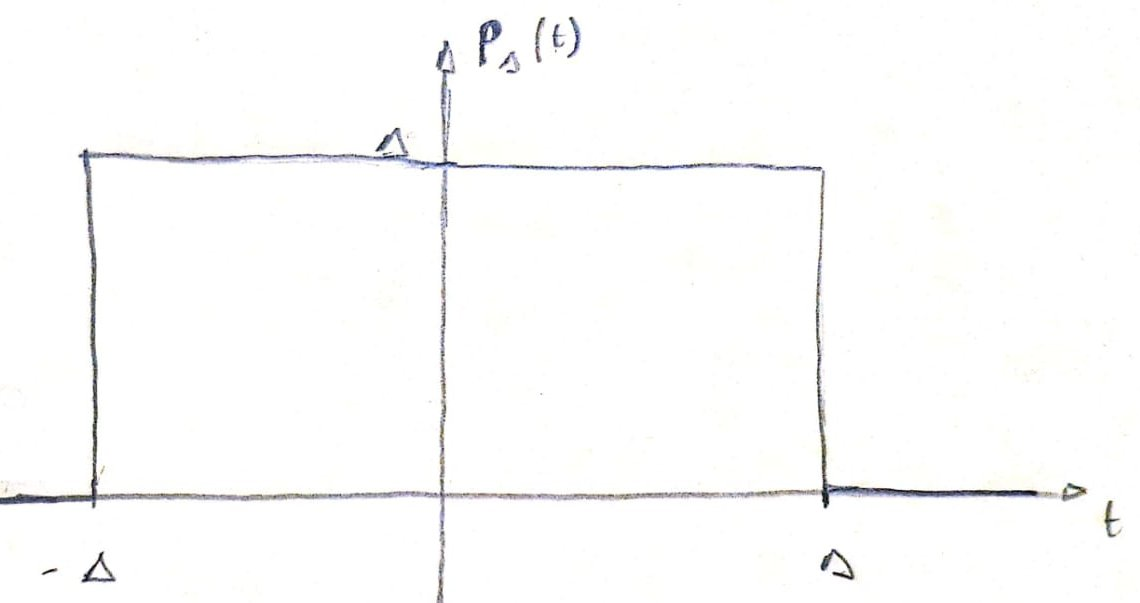
\includegraphics[scale=0.2]{questao2a1.jpeg}
        \centering
        \caption{$p_{\Delta}(t)$}
    \end{minipage}
    \begin{minipage}{9cm}
        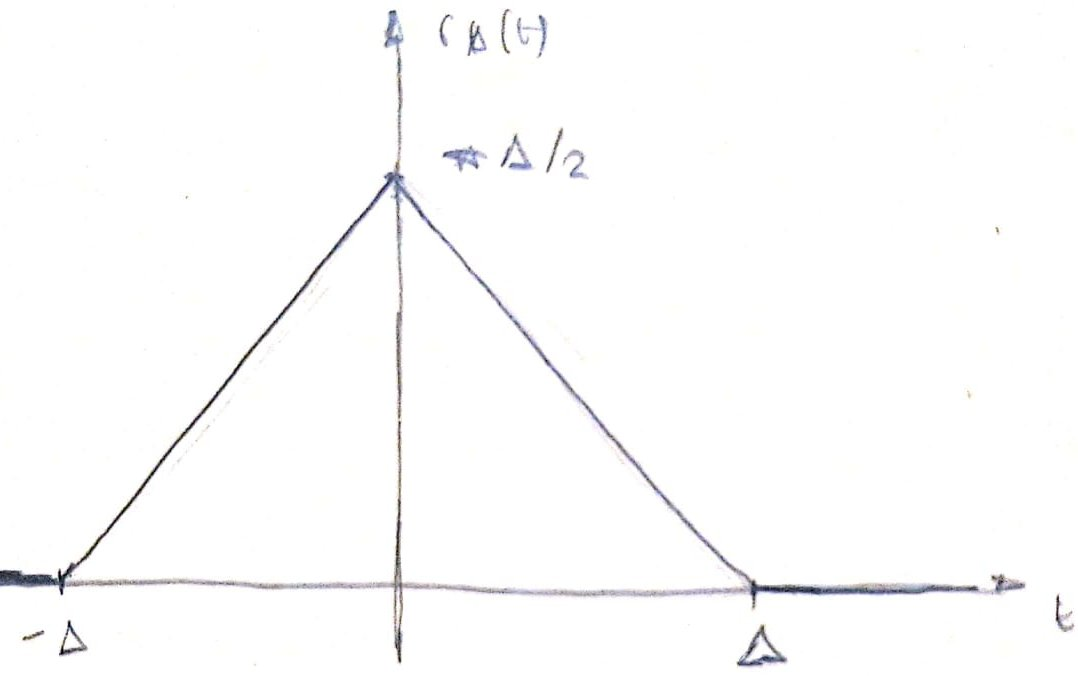
\includegraphics[scale=0.2]{questao2a2.jpeg}
        \centering
        \caption{$r_{\Delta}(t)$}
    \end{minipage}
    \begin{minipage}{9.5cm}
        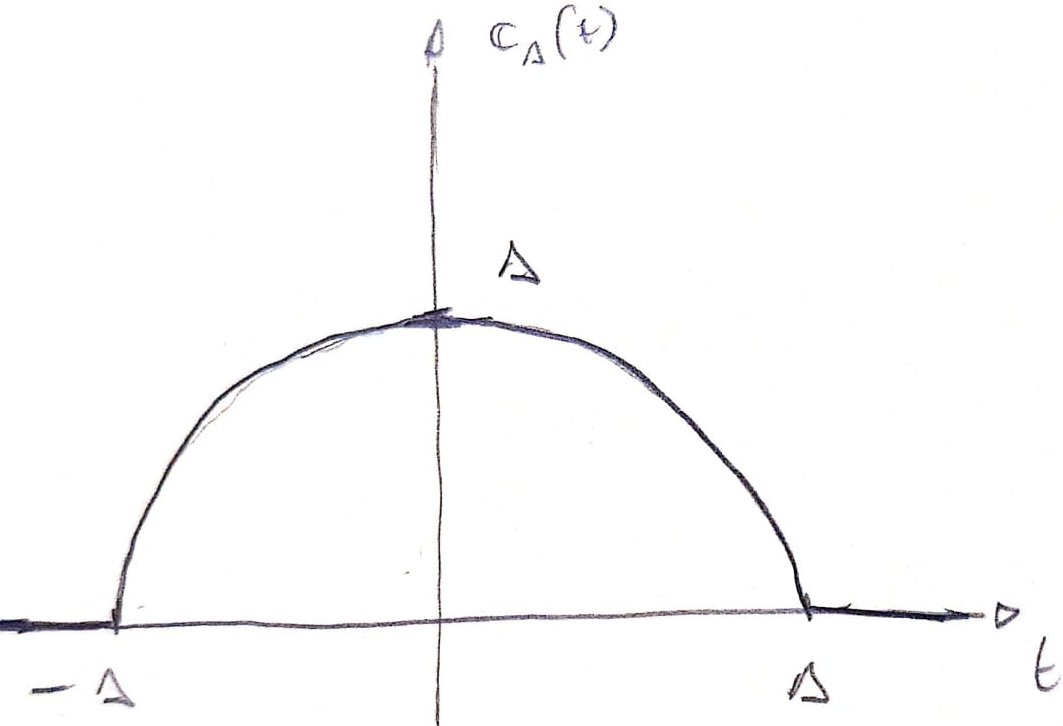
\includegraphics[scale=0.2]{questao2a3.jpeg}
        \centering
        \caption{$c_{\Delta}(t)$}
    \end{minipage}
    \begin{minipage}{9cm}
        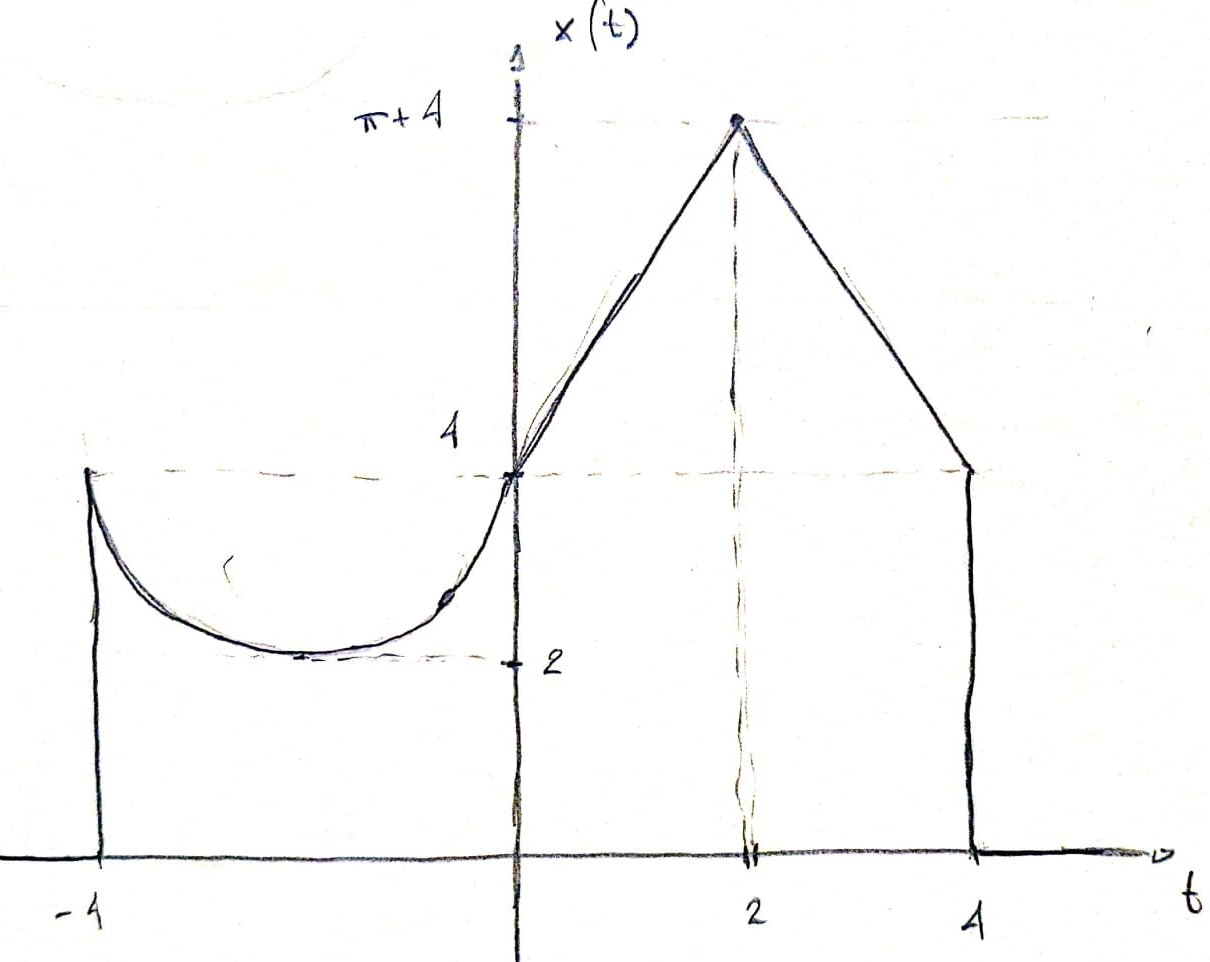
\includegraphics[scale=0.2]{questao2a4.jpeg}
        \centering
        \caption{$x(t)$}
    \end{minipage}   
\end{figure}

\newpage

(b) traçar o espectro de magnitude para $x(t)$, via FFT, determinando $T_0$ e $f_a$ por tentativa e erros;

\begin{figure}[h]
    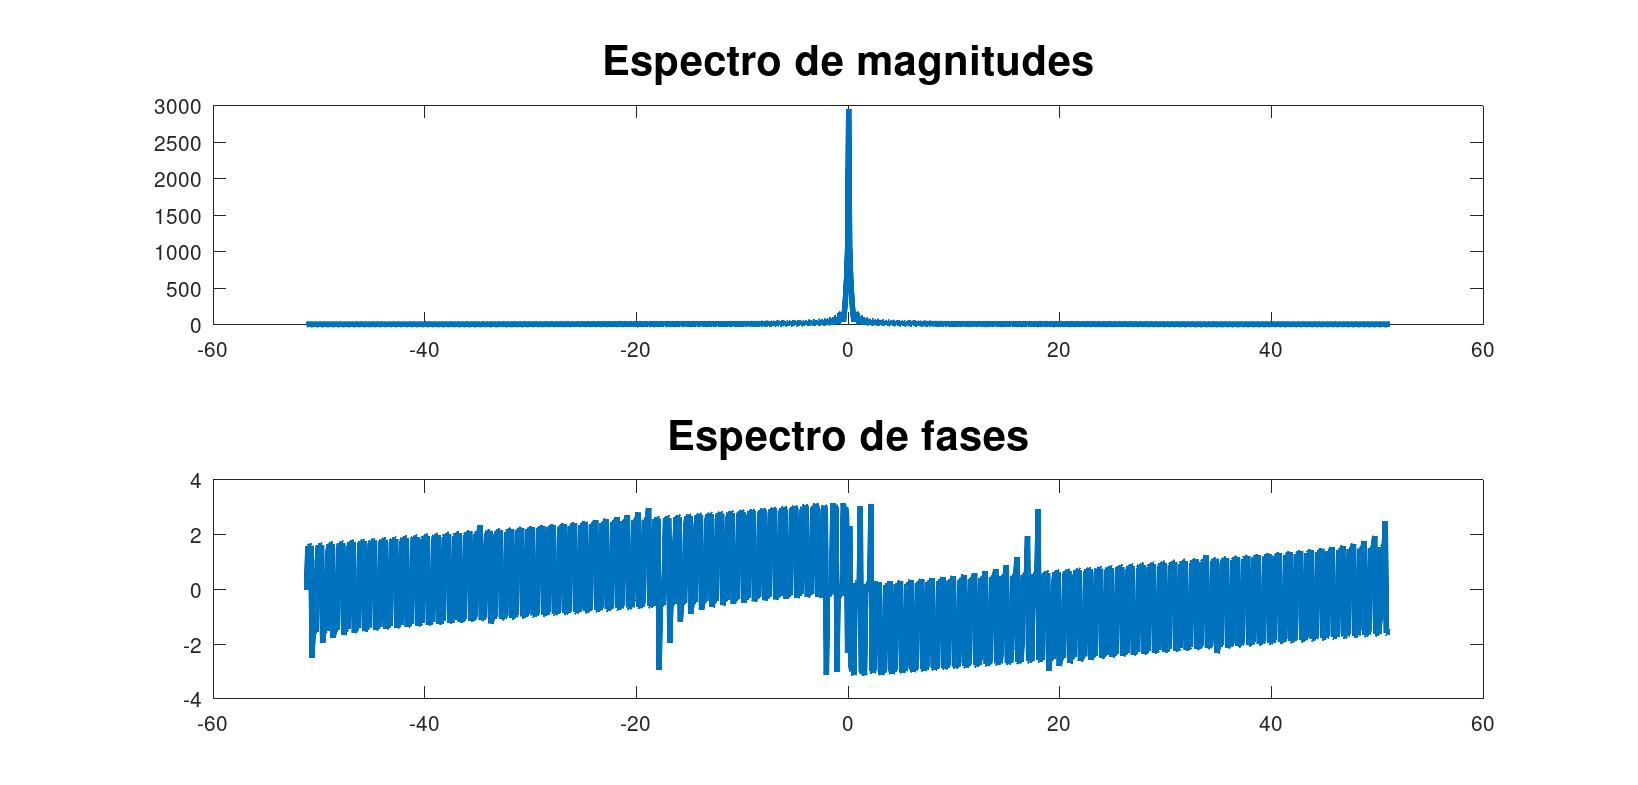
\includegraphics[scale=0.3]{plot2b.jpg}
    \centering
    \caption{Os espectros}
\end{figure}

(c) com a mesma janela, e o número de amostras aproximado para uma potência de 2, obter Haar 1;

\begin{figure}[h]
    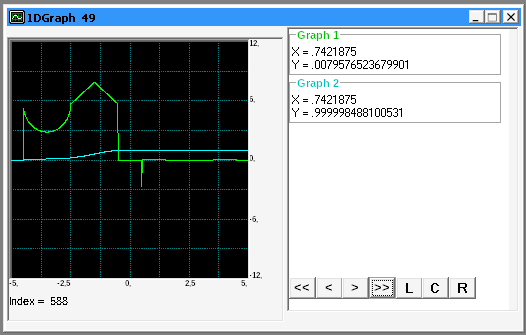
\includegraphics[scale=0.4]{plot2c.png}
    \centering
    \caption{Em verde, a transformada. Em azul, a energia.}
\end{figure}
O FAWAV, programa utilizado no caso, já utiliza uma amostragem de 1024 por padrão. A energia foi utilizada para traçar os outros gráficos.

(d) obter a Haar inversa do sinal truncado para reter $90.00\%$ da energia e plotar no mesmo gráfico;

\begin{figure}[h]
    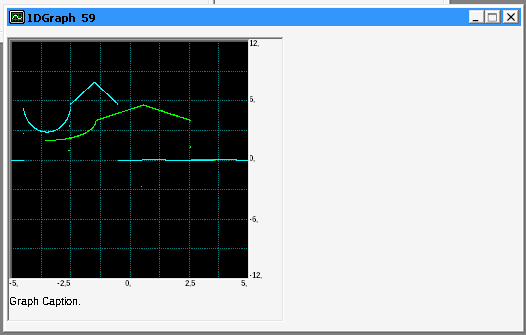
\includegraphics[scale=0.4]{plot2d.png}
    \centering
    \caption{Em azul, a transformada. Em verde, o sinal truncado}
\end{figure}

\newpage

(e) idem (d) para reter $99.99\%$ da energia e plotar no mesmo gráfico.

\begin{figure}[h]
    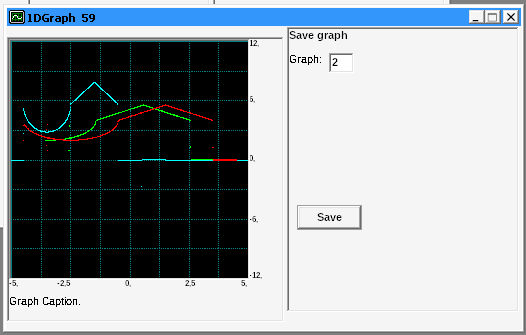
\includegraphics[scale=0.4]{plot2e.png}
    \centering
    \caption{Em azul, a transformada. Em verde, o sinal truncado para $90.00\%$. Em vermelho, o sinal truncado para $99.99\%$}
\end{figure}

\vspace{\baselineskip}

\textbf{3.)} Para o sinal a seguir:
\[x(t) = 8\sinc(4t) - 2\sinc(2t)\]

(a) plote o gráfico;

Abaixo, o código utilizado no octave:

\begin{verbatim}
%Questão 2.a)
% Intervalo
dt=0.025;
% Dados basicos
t=-5:dt:5-dt;
x=8*sinc(4*t)-2*sinc(2*t);
plot (t, x);
xlabel("t", "fontsize", 15);
ylabel("x(t)", "fontsize", 15);
\end{verbatim}

\begin{figure}[h]
    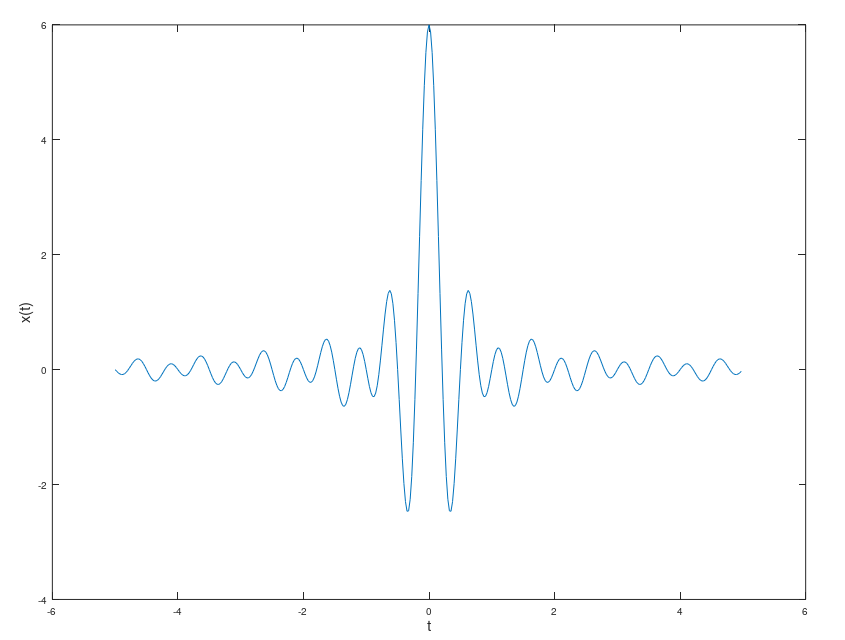
\includegraphics[scale=0.65]{questao3a}
    \centering
    \caption{Plotagem do gráfico - 3)}
\end{figure}

(b) encontre, justificando, a largura $T_0$ de uma janela de observação centrada na origem;

A largura escolhida foi de $T_0 = 10$, uma vez que, valores além desse intervalo
não contribuem de forma significativa para a energia total do sinal.
\vspace{\baselineskip}

(c) idem período de amostragem $\Delta t$ seguro;

O período de amostragem seguro escolhido foi de $\Delta{t} = 0.025$ pois $f_a = \frac{1}{\Delta{t}}$,
e a frequência de amostragem $\frac{f_a}{2} \ge \frac{w}{2\pi} = \frac{4\pi}{2\pi} = 2$.\\
$f_a \ge 4$ então $\Delta{t} \le 0.25$, satisfazendo o valor escolhido.
\vspace{\baselineskip}

(d) encontre o número de pontos $N = 2^p$;

Sabemos que $\Delta t = \frac{T_0}{N - 1}$. Então:
\begin{align*}
    \Delta t &= \frac{10}{N - 1}\\
    0.025 &= \frac{10}{N - 1}\\
    N - 1 &= \frac{10}{0.025}\\
    N &= 401
\end{align*}

(e) que limiar deve ser usado para reter $99.99\%$ da energia?;

Obtivemos haar 1, pelo FAWAV, obtendo o gráfico em verde, abaixo. Em seguida, truncamos para ter, aproxximadamente $99.99\%$ da energia.
\begin{figure}[h]
    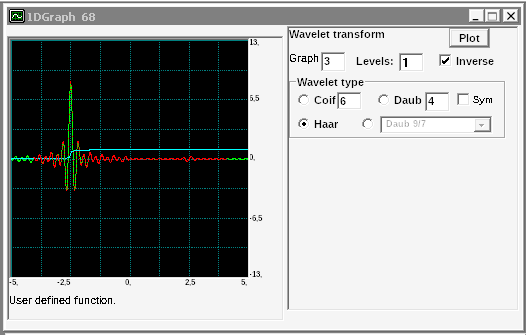
\includegraphics[scale=0.4]{plot3e.png}
    \centering
    \caption{}
\end{figure}

Fazendo a transformada inversa, obtivemos:
\begin{figure}[h]
    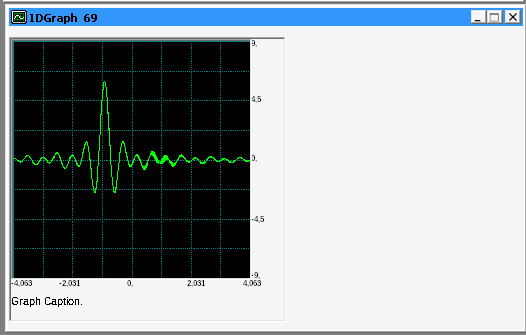
\includegraphics[scale=0.4]{plot3e2.png}
    \centering
    \caption{}
\end{figure}
O limiar, do gráfico ficou em $4.063$.

(f) que taxa de compressão isto produz? (Fazer para os níveis 1, 2, 3 e 10 de Haar, uma Daub qualquer de sua escolha e uma Coif qualquer de sua escolha);

\newpage

Para Haar 1:
\begin{figure}[h]
    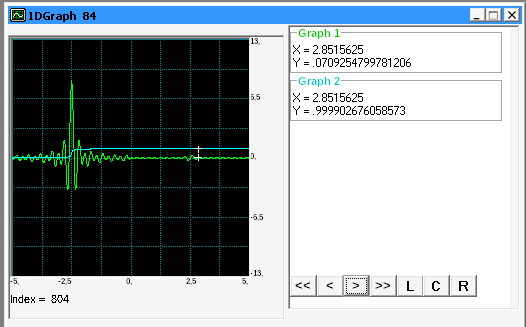
\includegraphics[scale=0.5]{haar1.png}
    \centering
    \caption{}
\end{figure}

Podemos retirar as amostras a partir de 804, restando (1024 - 804 = 220) amostras.

A taxa de compressão foi de $1024:220$ ou $256:55$.

Para Haar 2:
\begin{figure}[h]
    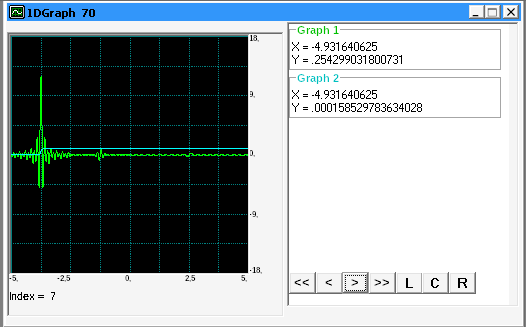
\includegraphics[scale=0.5]{haar2.png}
    \centering
    \caption{}
\end{figure}

Plotando a energia, de 1024 do todo, podemos retirar 7 intervalos do início e no fim, retirando ao todo, 14 intervalos.

A taxa de compressão foi de $512:7$

\newpage

Para Haar 3:
\begin{figure}[h]
    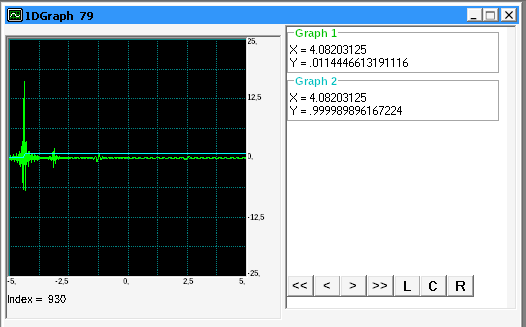
\includegraphics[scale=0.5]{haar3.png}
    \centering
    \caption{}
\end{figure}

Plotando a energia, de 1024 do todo, podemos retirar 93 amostras.

A taxa de compressão foi $1024:93$.

Para Haar 10:
\begin{figure}[h]
    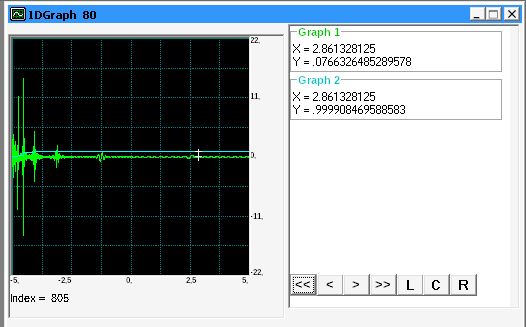
\includegraphics[scale=0.5]{haar10.png}
    \centering
    \caption{}
\end{figure}

Plotando a energia, de 1024 do todo, podemos retirar (1024 - 805 = 219) amostras.

A taxa de compressão foi $1024:219$.

\newpage

Para Doub 4 Nível 1:
\begin{figure}[h]
    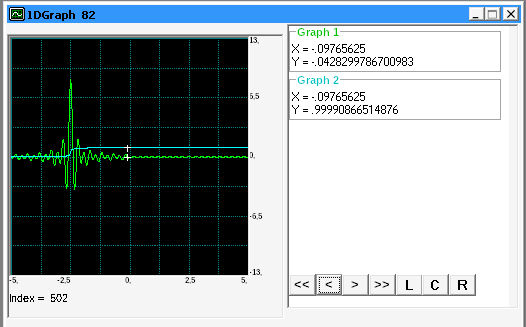
\includegraphics[scale=0.5]{doub1.png}
    \centering
    \caption{}
\end{figure}

Plotando a energia, de 1024 do todo, podemos retirar (1024 - 502 = 522) amostras.

A taxa de compressão foi $1024:522$ ou $512:261$.

Para Coif 6 Nível 1:
\begin{figure}[h]
    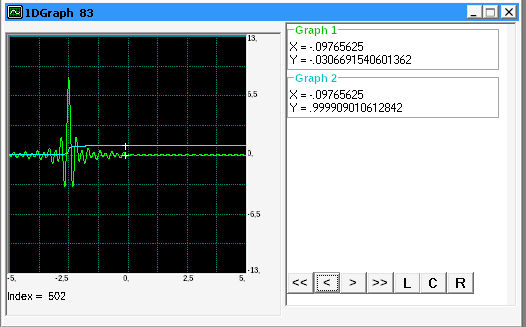
\includegraphics[scale=0.5]{coif 1.png}
    \centering
    \caption{}
\end{figure}

Plotando a energia, de 1024 do todo, podemos retirar (1024 - 502 = 522) amostras.

A taxa de compressão foi $1024:522$ ou $512:261$. A mesma que a Doub.

(g) comparar os resultados.

Em todos os casos que aparecem em ordem, a taxa de compressão sempre aumentava, mostrando como maiores níveis de Haar aumentam a eficiência, e que Doub e Coif são mais eficientes. Aqui, em Doub 4 e Coif 6, tivemos a mesma taxa de compressão.

\end{document}